\documentclass[tikz,dvipsnames]{standalone}
%\usepackage{tikz}
\usepackage{tikz-3dplot}
\usepackage{wasysym}

\begin{document}
\tdplotsetmaincoords{65}{130}
%
\pgfmathsetmacro{\rvec}{0.8}
\pgfmathsetmacro{\thetaJNvec}{40}
\pgfmathsetmacro{\thetaJLvec}{0}

\pgfmathsetmacro{\phivec}{20}
\pgfmathsetmacro{\phiNvec}{80}

\pgfmathsetmacro{\thetaA}{30}
\pgfmathsetmacro{\thetaB}{30}

\pgfmathsetmacro{\phiA}{20}
\pgfmathsetmacro{\phiB}{100}

\pgfmathsetmacro{\orbphase}{80}
%\pgfmathsetmacro{\longascnode}{-148}
% \pgfmathsetmacro{\longascnode}{-148-180}
\pgfmathsetmacro{\longascnode}{0}

\pgfmathsetmacro{\wfl}{\rvec}
\newcommand{\wfcolor}{gray}

\pgfmathsetmacro{\psil}{\wfl}
\pgfmathsetmacro{\psivec}{-30}

\pgfmathsetmacro{\orbitl}{0.5*\psil}

\pgfmathsetmacro{\discrad}{0.8*\rvec}

\pgfmathsetmacro{\phiNvec}{80}

\newcommand*\lateraleye{%
\scalebox{0.25}{
\tikzset{every picture/.style={line width=0.75pt,-}} 
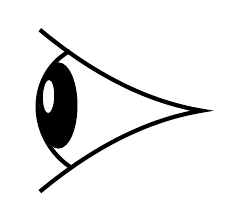
\begin{tikzpicture}[x=0.75pt,y=0.75pt,yscale=-1,xscale=1]
\draw  [-,line width=1.5]  (300,100.33) .. controls (326,122) and (352,135) .. (378,139.33) .. controls (352,143.67) and (326,156.67) .. (300,178.33) ;
\draw  [-,fill={rgb, 255:red, 0; green, 0; blue, 0 }  ,fill opacity=1 ] (308.94,116.33) .. controls (313.87,116.33) and (317.86,125.51) .. (317.85,136.83) .. controls (317.84,148.15) and (313.84,157.33) .. (308.91,157.33) .. controls (303.99,157.32) and (300,148.14) .. (300.01,136.82) .. controls (300.02,125.5) and (304.02,116.32) .. (308.94,116.33) -- cycle ;
\draw  [-,draw opacity=0][line width=1.5]  (314.84,166.6) .. controls (311.87,164.64) and (309.14,162.18) .. (306.76,159.24) .. controls (295.12,144.82) and (296.6,124.33) .. (310.07,113.45) .. controls (311.48,112.32) and (312.96,111.33) .. (314.5,110.49) -- (331.14,139.55) -- cycle ; \draw  [line width=1.5]  (314.84,166.6) .. controls (311.87,164.64) and (309.14,162.18) .. (306.76,159.24) .. controls (295.12,144.82) and (296.6,124.33) .. (310.07,113.45) .. controls (311.48,112.32) and (312.96,111.33) .. (314.5,110.49) ;
\draw  [-,fill={rgb, 255:red, 255; green, 255; blue, 255 }  ,fill opacity=1 ] (304.43,124.2) .. controls (306.09,124.25) and (307.32,128.01) .. (307.18,132.6) .. controls (307.05,137.19) and (305.59,140.88) .. (303.93,140.83) .. controls (302.27,140.78) and (301.03,137.02) .. (301.17,132.43) .. controls (301.31,127.83) and (302.76,124.15) .. (304.43,124.2) -- cycle ;
\end{tikzpicture}
}\,}

%
\begin{tikzpicture}[scale=5,tdplot_main_coords]
    \coordinate (O) at (0,0,0);
    \coordinate (m1) at ({\discrad*cos(90-\phiNvec)},{-\discrad*sin(90-\phiNvec)},0);

    \draw[thick,->, black] (O) -- ({\rvec*cos(90-\phiNvec)},{-\rvec*sin(90-\phiNvec)},0) node[anchor=north]{$\hat{x}_L$};
    \draw[thick,->, black] (O) -- ({\rvec*cos(\phiNvec)},{\rvec*sin(\phiNvec)},0) node[anchor=north]{$\hat{y}_L$};
    \draw[thick,->] (0,0,0) -- (0,0,\rvec) node[anchor=south]{$\hat{z}_L = \hat{L}$};

    \tdplotsetcoord{J}{\rvec}{0}{0}

    \draw[fill=gray,opacity=0.2] (\discrad,0,0) arc (0:360:\discrad);
    \draw[thin,opacity=0.5] (\discrad,0,0) arc (0:360:\discrad);

    % SPIN A

    \tdplotsetthetaplanecoords{\phiA}
    \tdplotdrawarc[tdplot_rotated_coords,NavyBlue]{(0,0,0)}{0.5}{0}%
            {\thetaA}{anchor=south, xshift=-2pt, yshift=2pt}{$\theta_{1}$}

    \tdplotsetrotatedcoords{\phiA}{\thetaA}{0}
    \draw[very thick,tdplot_rotated_coords,->, NavyBlue, opacity=1] (0,0,0)
        -- (0,0,\wfl) node[anchor=south east]{$\hat{S}_1$};

    \tdplotsetcoord{L}{\wfl}{\thetaA}{\phiA}
    \draw[thick,dotted, color=NavyBlue] (O) -- (Lxy);
    \draw[thick,dotted, color=NavyBlue] (L) -- (Lxy);
    \tdplotdrawarc[NavyBlue]{(O)}{0.3}{\phiNvec-90}{\phiA}{anchor=north east}{$\phi_{1}$}

    % SPIN B

    \tdplotsetthetaplanecoords{\phiB}
    \tdplotdrawarc[tdplot_rotated_coords,OliveGreen]{(0,0,0)}{0.5}{0}%
            {\thetaA}{anchor=south, xshift=-2pt, yshift=2pt}{$\theta_{2}$}

    \tdplotsetrotatedcoords{\phiB}{\thetaB}{0}
    \draw[very thick,tdplot_rotated_coords,->, OliveGreen, opacity=1] (0,0,0)
        -- (0,0,\wfl) node[anchor=south east]{$\hat{S}_2$};

    \tdplotsetcoord{L}{\wfl}{\thetaB}{\phiB}
    \draw[thick,dotted, color=OliveGreen] (O) -- (Lxy);
    \draw[thick,dotted, color=OliveGreen] (L) -- (Lxy);
    \tdplotdrawarc[OliveGreen]{(O)}{0.2}{\phiNvec-90}{\phiB}{anchor=north}{$\phi_{2}$}

\end{tikzpicture}
\end{document}
